\chapterimage{head2.png} % Chapter heading image
\chapter{Introduction}
\label{ch:introduction}
Nature's change and evolution is produced by the dynamics that governs bodies and systems contained in the Universe. All the known interactions can be described in terms of the four Fundamental Forces: gravitation, weak, electromagnetic and strong in ascending order of relative strength. High Energy Physics was able to describe the weak, electromagnetic and strong forces in terms of a $SU(3)\times SU(2)\times U(1)$ gauge symmetry group in what is known as the {\it Standard Model} \cite{halzen1984quarks,peskin1995introduction,weinberg1995quantum,weinberg1996quantum,2000hep.ph....1283N}. Nevertheless, attempts to include Gravitation in a similar frame has not provided yet satisfactory results.
\newline

The current consensus theory of gravitation is Einstein's General Relativity, that describes gravity as a deformation of the space-time. It is based on two assumptions: physical laws must be the same in every the coordinate system (Principle of Covariance) and Special Relativity must hold locally for every inertial observer (Principle of Equivalence). The most general second-order differential equation that holds these principles is the Einstein's field equation \cite{ANDP:ANDP19163540702,1916AnP...354..769E,1917SPAW.......142E,2001LRR.....4....1C}
\begin{equation}
R_{\mu\nu}-\frac{1}{2}Rg_{\mu\nu} + \Lambda g_{\mu\nu} = \frac{8\pi G_N}{c^4}T_{\mu\nu},
\label{eq:einsteinbare}
\end{equation}
where $R_{\mu\nu},T_{\mu\nu}$ are the Ricci and energy-momentum tensor respectively, $c$ the speed of light and $R=g^{\mu\nu}R_{\mu\nu}$ is the Ricci scalar. The free parameters of this equation are $G_N$ --Newton's constant-- and $\Lambda$, the cosmological constant.
\newline

Previous equation can also be obtained on the variational formalism using the Einstein-Hilbert action \cite{Hilbert:1915tx}:
\begin{equation}
S = \frac{c^4}{16\pi G_N}\int d^4x\sqrt{-g}(R-2\Lambda)+S_M,
\label{eq:ehaction}
\end{equation}
with $S_M$ the matter term of the action and $g=\det(g_{\mu\nu})$.

\section{The $\Lambda$CDM Cosmology}
One of the consequences of Einstein's equation is that the metric tensor is not static, implying that the geometry of the Universe changes. Thus, the space-time is a dynamical entity itself and its past and future evolution can be computed withing the framework of General Relativity.
\newline

Assuming that the Universe is homogeneous and isotropic \citep{2014MNRAS.440...10A,2015MNRAS.449..670A}, the only possible metric tensor is the Friedman-Lema\^itre-Robertson-Walker metric (FLRW) given by the line element \cite{1927ASSB...47...49L}
\begin{equation}
ds^2 = -dt^2+a^2(t)\left[\frac{dr^2}{1-Kr^2}+r^2(d\theta^2+\sin^2\theta d\phi^2)\right],
\end{equation}
where $a(t)$ is a function of time know as scale factor, $K=-1,0,1$ is the curvature of the universe and $r,\theta,\phi$ are the spatial 3D spherical coordinates.
\newline

Solving Einstein's equation for this metric, an expression for the evolution of the scale factor with time can be obtained
\begin{equation}
H^2(t)\equiv \left[\frac{\dot a(t)}{a(t)}\right]^2 = \frac{8\pi G_N}{3c^4}\rho(t) -\frac{K}{a^2(t)},
\end{equation}
where the dot denotes time derivatives, and $\rho$ is the total density of energy. The parameter $H$ has been defined as the expansion rate and its value at present $H_0$ is known as Hubble's constant.
\newline

Expansion rate can be expressed in terms of the normalized energy densities
\begin{equation}
H^2(t) = H_0^2\left[\sum_i\Omega_i(t)-\Omega_K\right]
\label{eq:flrw}
\end{equation}
with
\begin{equation}
\Omega_K\equiv\frac{K}{[a(t)H_0]^2}\ \ \mbox{ and }\ \ \Omega_i(t)\equiv \frac{8\pi G_N\rho_i(t)}{3H_0^2}.
\end{equation}
The parameter $\Omega_i$ is the density of the $i$-th matter/energy specie whose evolution with time can be computed using Thermodynamics. For non-relativistic matter --that is, matter with velocity $v\ll c$--, 
\begin{equation}
\Omega_M(t) = \Omega_M^0a^{-3}(t),
\end{equation}
whereas for relativistic matter species --that is, $v\sim c$--
\begin{equation}
\Omega_r(t) = \Omega_r^0 a^{-4}(t).
\end{equation}
Here $\Omega_i^0$ denotes the value on the present day of the $i$-th matter specie and, by construction, the following equation holds:
\begin{equation}
\sum_i\Omega_i^0=1+\Omega_K.
\label{eq:conservationenergy}
\end{equation}
Taking into account that the matter species and the curvature evolve on a different manner with time (\autoref{fig:rho_de}), its relative abundance at present fixes the expansion rate for the whole history of the Universe from birth to death.
\begin{figure}
\begin{center}
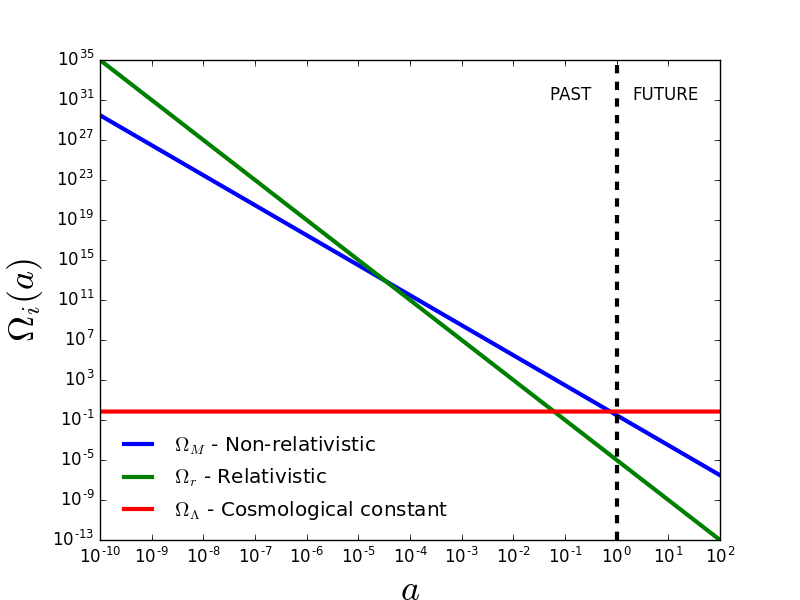
\includegraphics[width=0.85\textwidth]{./Pictures/rho_a.png}
\caption{Critical energy density for different types of matter species as function of the scale parameter of the Universe: relativistic (cold matter), non-relativistic (radiation), and cosmological constant. It can be seen that at present (black-dashed line), cosmological constant has just started to be dominant over the other species.}
\label{fig:rho_de}
\vspace*{0.2cm}
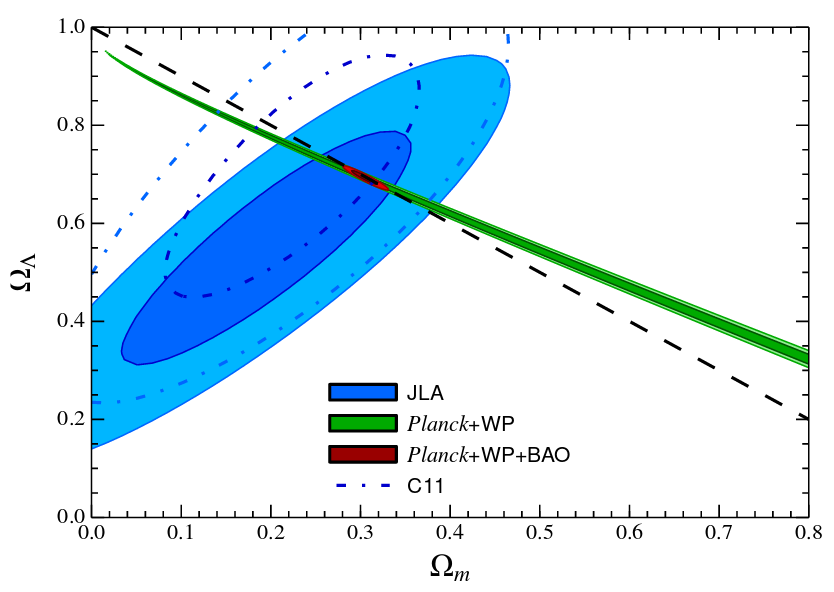
\includegraphics[width=0.8\textwidth]{./Pictures/om_ol.png}
\caption{Determination of the non-relativistic matter and dark energy content of the universe with the combination of SNIa, BAO, CMB from \cite{2014A&A...568A..22B}.}
\label{fig:om_ol}
\end{center}
\end{figure}
\newline

General Relativity with FLRW metric constitutes the theoretical basis for the current fiducial cosmological model: $\Lambda$CDM. It states that the Universe is flat, homogeneous and isotropic; has a non-zero cosmological constant and its non-relativistic matter content is mainly composed by what is known as dark matter. Dark matter is a form of matter that is not on the Standard Model of High Energy Physics and interacts with the ordinary --a.k.a. baryonic-- matter trough gravity (\autoref{fig:bullet}). Latest constrains on the density of the different matter species by Planck Collaboration 2015 \cite{2015arXiv150201589P} can be found at \autoref{tab:lcdm_parameters}.
\begin{table}
\begin{center}
\begin{tabular}{c | c | c | c }
$\Omega_M$ & $\Omega_\Lambda$ & $\Omega_b$ & $\Omega_K$\\
\hline
$0.315\pm 0.013$ & $0.685\pm 0.013$ & $0.04904\pm 0.00051$ & $-0.0001\pm 0.0052$\\
\end{tabular}
\caption{Density at present of the different matter species according to Planck 2015 \citep{2015arXiv150201589P}.}
\label{tab:lcdm_parameters}
\end{center}
\end{table}
\begin{figure}
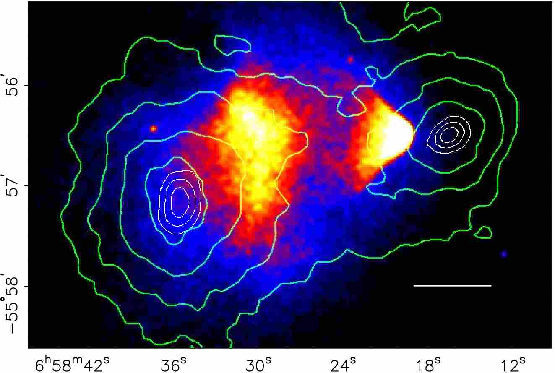
\includegraphics[width=\textwidth]{./Pictures/bullet_cluster.png}
\caption{Bullet cluster. Colors indicate the baryonic mass measured with gamma-rays, whereas the solid lines indicate the mass reconstructed with gravitational lensing. This result is considered the clearest evidence that baryonic- and dark-matter are decoupled. Image taken from \cite{2008PhRvD..78j4004D}.}
\label{fig:bullet}
\end{figure}

\section{The Cosmological Constant problem}
The cosmological constant can be absorbed on the right-hand-side of the \autoref{eq:einsteinbare} and interpreted as a constant matter term known as dark energy:
\begin{equation}
R_{\mu\nu}-\frac{1}{2}Rg_{\mu\nu} = \frac{8\pi G_N}{c^4}T_{\mu\nu}-\Lambda g_{\mu\nu}.
\end{equation}
With this matter term, assuming $\Omega_K=0$, \autoref{eq:flrw} transforms into
\begin{equation}
H^2(t) = H_0^2\left[\sum_i\Omega_i(t) +\Omega_\Lambda(t)\right],
\end{equation}
where $\Omega_\Lambda(t)=\Omega_\Lambda^0$ is the dark energy density. This new term is a time-independent constant that has the same value on every location of the Universe. Thus, as the other matter species has a density that decreases with time, the dark energy density has only impact at late cosmic times.
\newline

This new term may be regarded as a new matter specie such that
\begin{equation}
\rho_\Lambda = \frac{3H_0^2}{8\pi G_N}\Omega_\Lambda.
\label{eq:rho_lambda}
\end{equation}
Taking into account \autoref{eq:conservationenergy} and \autoref{eq:rho_lambda}, an upper bound on the dark energy density can be established
\begin{equation}
\rho_\Lambda \leq \frac{3H_0^2}{8\pi G_N} \sim 10 ^{-47} \mbox{ GeV}^4.
\label{eq:cosmologicalconstant}
\end{equation}
\newline

Since this energy density fills the whole Universe and is an inherent property of the geometry of the Universe and hence of the Universe itself, from a physical point of view it can be identified as the energy of the vacuum \cite{RevModPhys.61.1,2003PhR...380..235P,PhysRevD.72.021301}. Quantum Field Theory (QFT) states that the quantum vacuum is not empty and static but it actually is a dynamical entity. Assuming that the Standard Model is valid up to the Planck scale, the energy density of the vacuum can be estimated to be
\begin{equation}
\rho_{QFT} = \int\limits_0^{1/L_P} dk \sqrt{k^2+m^2}\frac{4\pi k^2}{(2\pi)^4}\sim 10^{71}\mbox{ GeV}^4,
\end{equation}
where $L_P$ is Planck's length. Thus, there's a miss-match between the amount of dark energy measured and that predicted by QFT of many orders of magnitude. It can be argued that although it is known that Planck's energy scale is the upper range of validity of Standard Model physics, nothing prevents that it starts to fail at lower scales. A lower bound on this point can be established as the Quantum Cromodynamics (QCD) cutoff scale ($\sim 200$ MeV), leading to a vacuum energy density of
\begin{equation}
\rho_{QCD} = \int\limits_0^{1/L_{QCD}} dk \sqrt{k^2+m^2}\frac{4\pi k^2}{(2\pi)^4}\sim 10^{-3}\mbox{ GeV}^4,
\end{equation}
reducing the tension between theory and experiment, but still being catastrophic. It is worth to remark that establishing the range of validity of the Standard Model at the QCD cutoff scale is an optimistic scenario for the cosmological constant, since latest LHC results have demonstrated its validity of the Standard Model up to 1 TeV.
\newline

It can be argued that the cosmological constant is not connected to High Energy Physics. Nevertheless, the energy of the quantum vacuum is still there and must be taken into account, not solving the discrepancy.


\section{Theories for Dark Energy}
As it has been stated previously, the small value of the cosmological constant can not be explained with the Standard Model of High Energy Physics. Thus, one can force the cosmological constant to be $\Lambda=0$ and try to explain accelerated expansion of the Universe with other class of theories. The simplest approach is to postulate the existence of new exotic matter that has a negative pressure that drives the accelerated expansion. The other approach consist on postulating a new gravitational field equation by modifying Einstein's equation or starting from scratch.

\subsection{Exotic matter fields}
An explanation to the accelerated expansion of the Universe can be found on the presence on new quantum fields. The simplest case is known as quintessence and is defined as a scalar field  ($\phi$) that is added to the action defined at \autoref{eq:ehaction} such that
\begin{equation}
S = \frac{c^4}{16\pi G_N}\int d^4x\sqrt{-g}R+S_\phi+S_M
\end{equation}
with
\begin{equation}
S_\phi = \int d^4x\left[\frac{1}{2}g^{\mu\nu}\partial_\mu\phi\partial_\nu\phi-V(\phi)\right],
\end{equation}
where $V(\phi)$ is the potential of the field. On the FLRW metric, this leads to a substance with pressure and density respectively 
\begin{equation}
P_\phi = \frac{1}{2}\dot\phi^2-V(\phi)\ \ \mbox{ and }\ \ \rho_\phi=\frac{1}{2}\dot\phi^2+V(\phi).
\end{equation}
This can be parametrized as an ideal fluid with equation of state
\begin{equation}
w_{DE} = \frac{P_\phi}{\rho_\phi} = \frac{\dot\phi^2-2V(\phi)}{\dot\phi^2+2V(\phi)}.
\end{equation}
Thus, it can be deduced that dark energy density evolves with the scale factor of the universe as
\begin{equation}
\Omega_\Lambda(t) = \Omega_\Lambda^0 [a(t)]^{-3(1+w_\phi)}.
\end{equation}
\newline

The only possible candidate for dark energy as quintessence within the Standard Model of Particle Physics is the Higgs field, a complex scalar-field that fills the Universe and couples to gauge bosons giving them its mass. The potential of the field is given by
\begin{equation}
V(\phi) = \mu_H^2\phi^\dagger\phi+\frac{1}{4}\lambda_H(\phi^\dagger\phi)^2,
\end{equation}
with $\mu_H$ the mass term, $\lambda_H$ the self-interaction of the field and $\phi,\phi^\dagger$ the Higgs field and its hermitian conjugate respectively. Since the potential of the field is time independent, this leads to an equation of state
\begin{equation}
w_{DE} = \frac{-2V(\phi)}{2V(\phi)} = -1,
\end{equation}
recovering the cosmological constant solution. Thus, the cosmological constant can also be interpreted alternatively as the expected value of Higgs field at vacuum
\begin{equation}
\langle 0|\phi_0|0\rangle = \frac{|\mu_H|}{\sqrt{\lambda_H}}= \sqrt{\frac{1}{\sqrt{2}G_F}}= 246\mbox{ GeV}^4,
\end{equation}
not solving the discrepancy of several orders of magnitude with the cosmological constant energy density as given by \autoref{eq:cosmologicalconstant}. Here $G_F$ is the Fermi constant, that can be computed from the decay of the muon. The connection between the decay of the muon and the Higgs field comes from the fact that the decay is mediated by vector bosons, whose mass is given by the Higgs field:
\begin{equation}
\mu^- \rightarrow W^- + \nu_\mu \mbox{ and }W^-\rightarrow e^-+\bar\nu_e.
\end{equation}
\newline

Other High Energy Physics potentials can be built from physics beyond the Standard Model, such us supergravity and supersymmetry \cite{1999PhLB..468...40B,1999astro.ph.12005B,2000PhRvD..61j3502B,1999PhRvD..60f3502B}, where different scalar potential can be found. Even more complicated theories with more fields that may interact between them can be postulated and will not be considered here since they are beyond the scope of this Thesis. A detailed description of all the models can be found at \cite{2010deto.book.....A}. Nevertheless, a general phenomenological description can be made in terms of the equation of state of dark energy,
\begin{equation}
P_{DE} = w_{DE}\rho_{DE}
\end{equation}
expanding the parameter $w_{DE}$ in a power series of the scale factor
\begin{equation}
w_{DE}(t) = w_0 +w_a[1-a(t)],
\end{equation}
where $w_0$ denotes the value of the equation of state parameter at present and $w_a$ is evolution --at first order-- with time. The cosmological constant may be considered as an specific solution of this equation of state where
\begin{equation}
w_0=-1\ \ \mbox{ and }\ \ w_a=0.
\end{equation}
The key difference between the cosmological constant and exotic forms of matter is that the latter theories provide a dark energy density that evolves trough the cosmic history.

\subsection{Modified Gravity}
Attempts to explain the existence of a cosmological constant from High Energy Physics side lead to a tension between General Relativity and the Standard Model. Possible new exotic fields that may explain late-time cosmic acceleration are walking a tightrope due to latest LHC results \cite{2015arXiv150603091B}. The remaining approach to explain the accelerated expansion of the Universe is to consider General Relativity as an approximate gravitational theory on the same way Newtonian gravity is the low-energy limit of Einstein's gravity. Extensions to General Relativity are known as modified gravity models.
\newline

In order to preserve the symmetries of General Relativity, the new field equations must be a function of the Ricci scalar. The most general class of those theories is known as $f(R)$ gravity \cite{2010LRR....13....3D,2010RvMP...82..451S}, and its approach is to let the action to be a general function ($f$) of the Ricci scalar:
\begin{equation}
S = \frac{c^4}{16\pi G_N}\int d^4x\sqrt{-g}f(R),
\end{equation}
that leads to the field equation
\begin{equation}
R_{\mu\nu}-\frac{1}{2}Rg_{\mu\nu}=\frac{8\pi G_N}{c^4}( T_{\mu\nu}+T_{\mu\nu}^R).
\end{equation}
This field equation is similar to \autoref{eq:einsteinbare} but has an additional term $T_{\mu\nu}^R$ that takes into account the additional curvature terms that can be modeled as a fluid on the same way as the energy-momentum tensor. The simplest case is $f(R) =R+\alpha R^n$ with $\alpha,n\in\mathbb{R}$, which has interesting cosmological solutions \cite{PhysRevD.85.083511}. This theory has very distinctive phenomenology such as double Einstein rings with just one source galaxy on an strong lens regime \cite{2011PhRvD..83b4030N} that --if found--, could be the smoking gun of these kind of theories. The existence of a double Einstein ring (SDSSJ0946+1006) has been reported \cite{2008ApJ...677.1046G}, nevertheless it is a system with one lens and two sources at different redshifts, producing one ring of different diameter each.
\newline

More complicated models of modified gravity that may break the equivalence principle and the Lorentz symmetry can be considered but are not going to be treated here since they are beyond of the scope of this Thesis. For a review it can be consulted \cite{2015CQGra..32x3001B}. The usual approach to explore the modifications to General Relativity \cite{2015PhRvD..91h3504L} is to consider the departures of the metric. On the Newtonian gauge, the FLRW line element of can be parametrized with the Newtonian and the lensing potential; $\Phi,\Psi$ respectively \cite{2015PhRvD..91h3504L}:
\begin{equation}
ds^2 = a^2(\tau)[-(1+2\Psi)d\tau^2+(1-2\Phi)dx_idx^j],
\end{equation}
with
\begin{equation}
2\nabla^2\Phi(a,k) = \frac{8\pi G_N}{c^2}a^2\mu(a,k)\bar \rho_M\delta_M(a,k)\ \ \mbox{ and }\ \ \gamma(a,k)=\frac{\Phi(a,k)}{\Psi(a,k)},
\end{equation}
where $\bar \rho_M$ is the average matter density, $\delta_M$ its fluctuations and $k$ is the wavenumber of the potentials. Here $\mu$ and $\gamma$ parametrize the departures from General Relativity, that is the specific case with
\begin{equation}
\mu(a,k) = 1\ \ \mbox{ and }\ \ \gamma(a,k) = 1.
\end{equation}

It is important to remark that the zoo of all the departures from General Relativity plus cosmological constant --including the addition of new fields--, may be unified into a single parametrization known as Parametrized Post-Friedmann Framework \cite{2013PhRvD..87b4015B}.

\section{Probes for Dark Energy}
The nature of Dark energy can be constrained using different cosmological probes \cite{Weinberg201387} by measuring the $w_0,w_a$ parameters of its equation of state or, conversely for modified gravity, the potentials $\Sigma,\gamma$. The determination of these parameters can be split in two classes of probes: geometrical and large-scale-structure tests.
\newline

Geometrical measurements exploit the fact that the distances measured on cosmological scales depend on the metric tensor of the Universe, that is affected by the energy content of the Universe and the gravitational theory used. These measurements include: the barion acoustic oscillation peak-scale (BAO), the SNIa distance-ladder, Alcock-Paczynski \cite{1979Natur.281..358A} tests and integrated Sachs-Wolfe (ISW) effect. On the other side, large-scale-structure probes are based on the measurement of the inhomogeneities of the matter density field at different moments of the cosmic history, which depend on the matter/dark-energy ration and gravitational theory used. They include: the cluster-count evolution with redshift, redshift-space-distortions (RSD), clustering, lensing and the cosmic microwave background (CMB).
\newline

The combination of different cosmological probes leads to more accurate measurements at the same time it breaks degeneracies on the determination of the cosmological parameters \cite{2006A&A...448..831Y,Weinberg201387}. Nevertheless, multiprobe cosmology suffer from the correlation of the different methodologies. In addition, if the different probes are provided by the same experiment, they must also take into account the correlation of the different sources of systematic errors \cite{2016arXiv160105779K,2016arXiv160701761S,2017MNRAS.465L..20S,2017arXiv170307786F}.  Thus, the inclusion of an specific measurement on a multiprobe analysis, that is highly correlated with other probes or is very noisy, this may no lead to a significant improvement of the cosmological constrain.
\newline

Weak-lensing magnification is a low signal-to-noise measurement with many sources of systematic errors \cite{2016MNRAS.455.3943H} that is produced by the same physical entity as the gg-lensing, which has higher signal-to-noise (see \autoref{ch:theory} also for a full explanation of magnification and gg-lensing). Thus, the inclusion of magnification on a multiprobe analysis does not lead to an effective improvement of the measurement. This requires the use of magnification on environments and regimes that other probes can not reach.
\newline

The strength of magnification is that it allows to measure directly the matter profile of the large-scale-structures that conform the Universe. The full matter structures of the Universe are only accessible trough gravitational lensing due to the presence of dark matter. Since dark matter is not visible and interacts only trough gravity, assumptions on how the visible- --baryonic- -- and dark- matter assemble together must be made on measurements other than gravitational lensing, introducing nuisances on the measurement. One of those structures are known as voids, which are the emptiest regions of the cosmic web (see \autoref{fig:2df}).
\begin{figure}
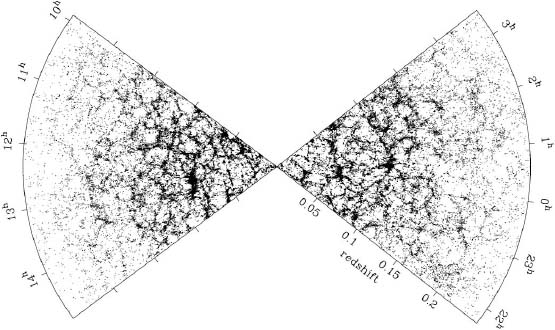
\includegraphics[width=\textwidth]{./Pictures/2df.jpg}
\caption{Large-scale-structure of the Universe. Each dot represents the position of a galaxy. Image credit: 2 Degree Field Survey.}
\label{fig:2df}
\end{figure}
\newline

Since voids have a lower matter content than the average Universe, their gravitational evolution is more dominated by dark energy. Thus, void properties are different depending on the dark energy properties. If the abundance of large voids on the Universe is considered, it has been reported that its number increases in $f(R)$ gravity models \cite{2012MNRAS.421.3481L} since the abundance of dark matter halos is altered \cite{2017JCAP...03..012V}. Nevertheless, if the shape of the void is measured, its ellipticity can be used as a probe for the parameters of the equation of state of dark energy \cite{2010MNRAS.403.1392L,0004-637X-754-2-109,PhysRevLett.98.081301,2013PhRvL.111x1103S}, since the structure growth-factor on the line-of-sight has a variation due to
the dark energy content, whereas on the transverse plane, growth-factor is constant. Finally, the radial distribution of matter around the center of a void --known as void profile-- has demonstrated to be different on $f(R)$ theories and General Relativity \cite{2014APh....54...44A,2014arXiv1410.8355C,2015MNRAS.451.4215Z,2015JCAP...08..028B,2016PhRvD..93j3522A,2016PhRvD..94j3524A}. Thus, by simply measuring the void matter profile, constrains on dark energy can be made.
\newline

Thus, the direct determination of the matter profile of voids by weak-lensing magnification, constitutes a promising and independent new probe on dark energy, alternative to multiprobe constrains.

\section{Current status of Dark Energy constrains}
The latest and more precise results constraining dark energy are provided by the Planck Collaboration 2015 results from the analysis of the Cosmic Microwave Background (CMB) \cite{2016A&A...594A..14P}.
\newline

Dark enery as an exotic form of matter, is determined by measuring the parameters of the equation of state ($w_0,w_a$) and their value can be seen at \autoref{fig:w0wa_planck2015}. Results are compatible with General Relativity plus cosmological constant, the uncertainty on the parameters of the equation of state does not allow to exclude many models, specifically the type of models that predict a value of the equation of state close to that of the cosmological constant but whose equation of state evolves with cosmic time --or equivalently, redshift--, since current precision on the determination of this evolution is still limited as it can be deduced from \autoref{fig:equationofstate_planck2015}. Constrains on Modified Gravity models are also given in terms of the modified gravity potentials $\mu,\eta$ and $\Sigma$.
\newline

\begin{figure}
\begin{center}
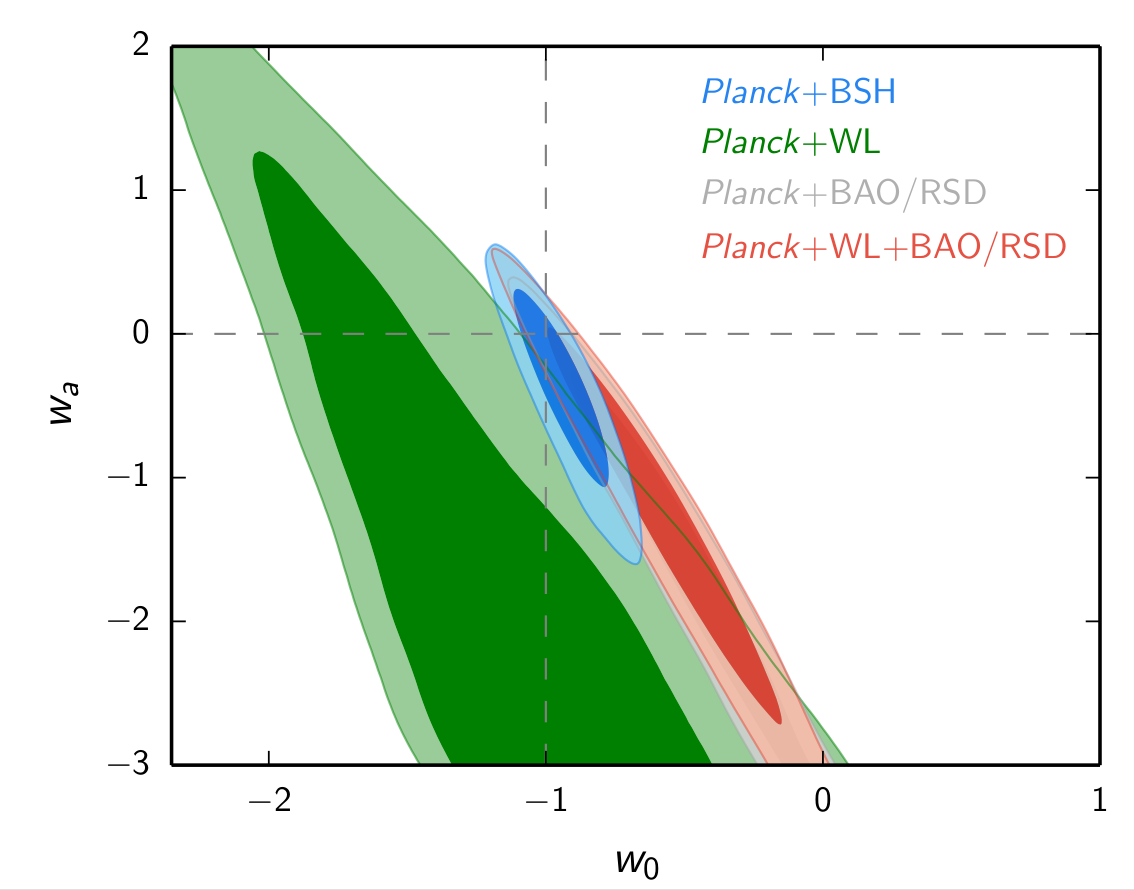
\includegraphics[width=0.8\textwidth,trim={0 3mm 0 0},clip]{./Pictures/w0wa_planck2015.png}
\caption{One- and two- sigma contours of the equation of state of dark energy $w_0,w_a$. The intersection of dashed lines is the cosmological constant. Results obtained from Planck Collaboration 2015 results \cite{2016A&A...594A..14P}.}
\label{fig:w0wa_planck2015}
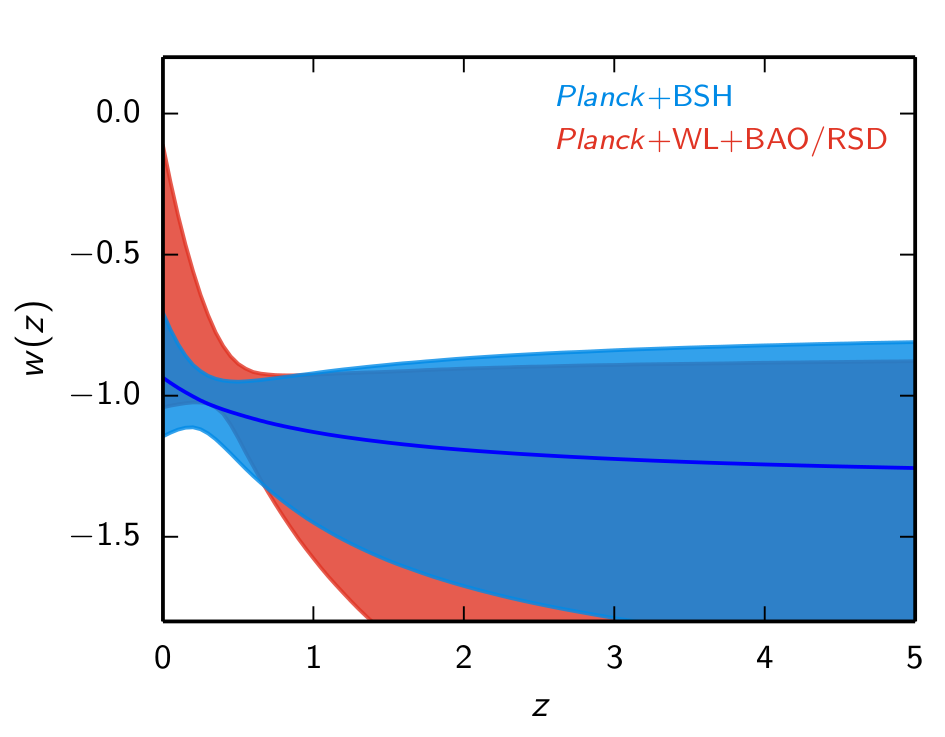
\includegraphics[width=0.8\textwidth]{./Pictures/equationofstate_planck2015.png}
\caption{One-sigma confidence interval of the equation of state of dark energy as a function of redshift $w_{DE}(z)$ and one-sigma confidence interval. Results obtained from Planck Collaboration 2015 results \cite{2016A&A...594A..14P}.}
\label{fig:equationofstate_planck2015}
\end{center}
\end{figure}

\begin{figure}
\begin{center}
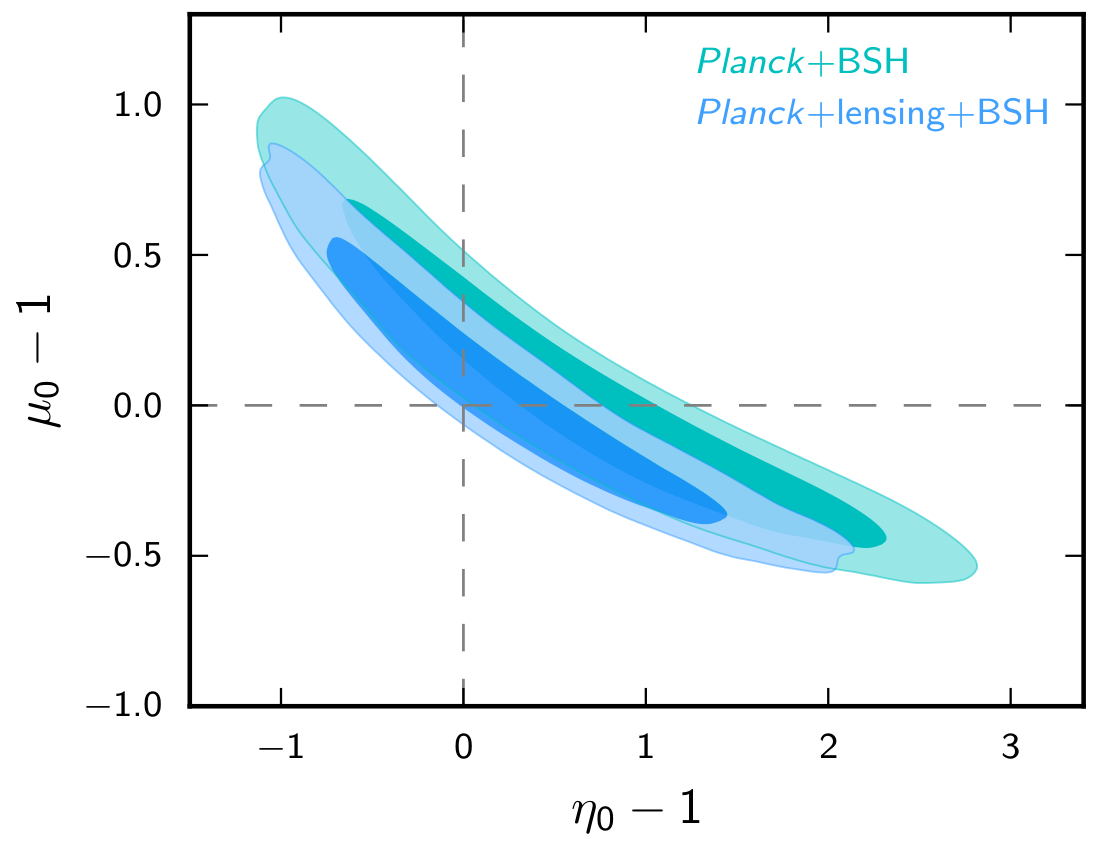
\includegraphics[width=0.8\textwidth]{./Pictures/mg_planck2015.png}
\caption{One- and two- sigma modified gravity potentials at present $\mu_0,\eta_0$. Dashed line is General Relativity plus cosmological constant. Results obtained from Planck Collaboration 2015 results \cite{2016A&A...594A..14P}.}
\label{fig:mg_planck2015}
\vspace*{0.2cm}
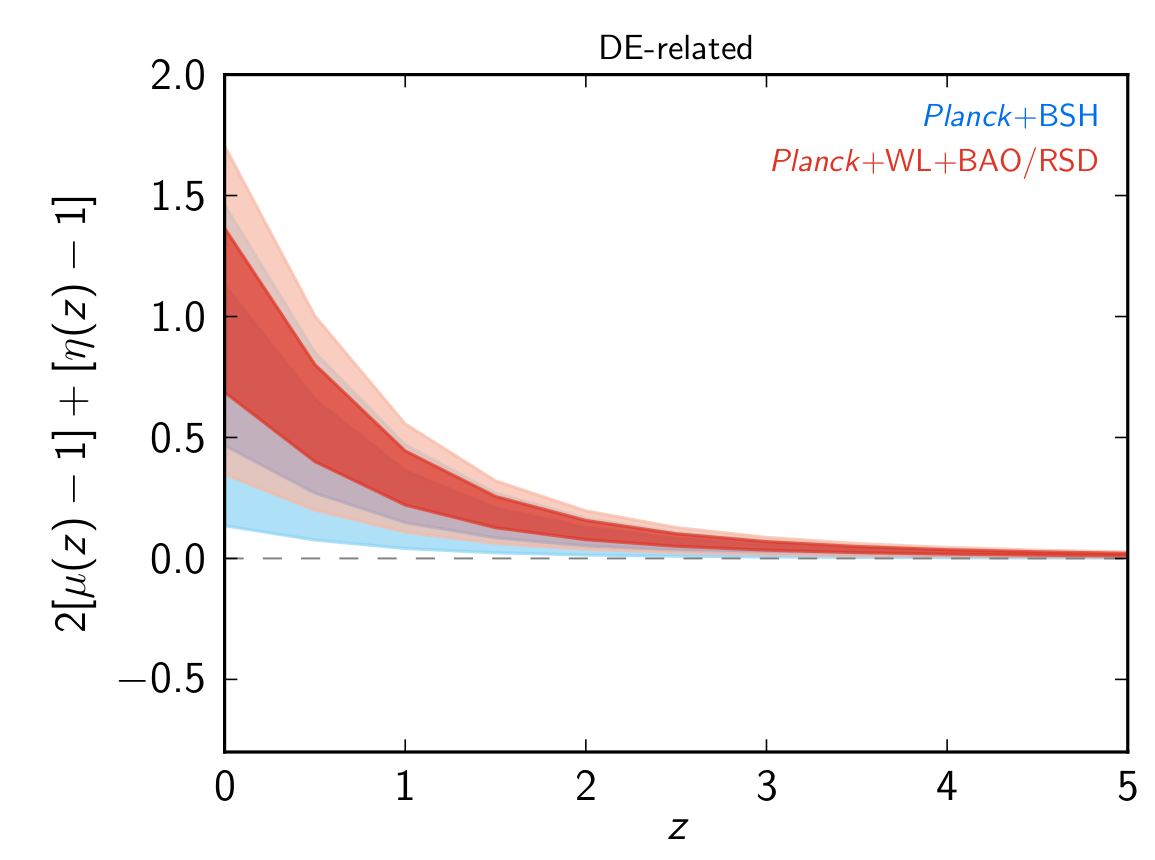
\includegraphics[width=0.8\textwidth]{./Pictures/munu_planck2015.png}
\caption{One- and two- sigma of the sum of the modified gravity potentials. Dashed line is General Relativity plus cosmological constant. Results obtained from Planck Collaboration 2015 results \cite{2016A&A...594A..14P}. }
\label{fig:munu_planck2015}
\end{center}
\end{figure}
The latest results from the Sloan Digital Sky Survey (SDSS) and its upgrade BOSS, provide several measurements that, although they do not constrain directly dark energy theories, show a good agreement with the flat-$\Lambda$CDM paradigm. These probes include: Alcock-Paczynski tests \cite{2016ApJ...832..103L}, the clustering of galaxies \cite{2016arXiv160703155A}, baryon acoustic oscillations (BAO) \cite{2016arXiv160703154W,2017arXiv170200176B} and redshift-space distortions \cite{2017MNRAS.465.1757G}.
\newline

Although the Planck Collaboration 2015 and SDSS/BOSS results agree between them and seem to favour cosmological constant as dark energy, there are some measurements that are in tension with Planck Collaboration 2015. 
\newline

Riess et~al. latest direct determination of the Hubble constant using the cosmological distance ladder (parallax-cepheids-SNIa) \cite{2016ApJ...826...56R}, show a discrepancy at the $3\sigma$ level with the Hubble constant measured by Planck Collaboration 2015.
\newline

CFHTLens \& KiDS-450 Collaborations weak gravitational lensing analysis show tension on the $\Omega_M-\sigma_8$ plane with Planck Collaboration 2013 \cite{2014A&A...571A..16P} and 2015 CMB measurements if a General Relativity plus cosmological constant scenario is considered \cite{2013MNRAS.430.2200K,2017arXiv170303383H}. This tension may be alleviated if other models are considered, such as non-zero curvature and dark energy models \cite{2016arXiv161004606J}. Nevertheless, discrepancies could also be produced by systematic effects \cite{2015PhRvD..92b3003D,2017MNRAS.465.2033J}.
\newline

A weak-lensing analysis by Leauthaud et~al. \cite{2017MNRAS.467.3024L} of CFHTLens \& CMASS data using weak gravitational lensing, show a lower signal amplitude that the one predicted measuring the clustering of the lens sample. In addition weak gravitational lensing measurements on the $\Omega_M^0-\sigma_8$ plane have a discrepancy on the $3\sigma$ level with Planck Collaboration 2013 measurements on a cosmological constant scenario. Nevertheless, discrepancies are interpreted in terms of new physics on the astronomy side: halo occupation distribution (HOD) and baryonic physics.
\newline

Recently, a dynamical dark energy scenario has shown to solve these tensions when combining severeal cosmological probes (weak-lensing, SNIa, BAO, and CMB) \cite{2017arXiv170108165Z}. An independent work has also shown that dynamical dark energy can solve these tensions combining Planck Collaboration 2015 with Riess et~al., SDSS BAO and CFHTLens measurements \cite{2017arXiv170400762D}. Nevertheless, constrains are still limited.
\newline

As it has been described, current individual constrains on dark energy are not precise enough to determine which model is the correct explanation of the accelerated expansion of the Universe. Nevertheless, current cosmological model --$\Lambda$CDM--, has demonstrated to be a solid theory that explains a wide range of physical effects and has passed the most stringent tests including gravitational waves \cite{1982ApJ...253..908T,PhysRevLett.116.061102}. Although a tension exists between different probes that may be alleviated in a  non-cosmological constant scenario, caution is needed and special attention is required to do a proper systematic error estimation. This requires additional probes and redundant measurements of the same physical observable but with different sources of systematic errors. We have entered in the precision cosmology era.
$$\S\qquad \S\qquad \S$$
This Thesis is devoted to the analysis of weak-lensing magnification as part of the Dark Energy Survey Collaboration. Data analysis is carried out on two different data-sets of the mentioned experiment with two different goals each. The first analysis is carried out on the Science Verification data-set, aiming the detection of the magnification signal and the development of new techniques of systematic error mitigation. Once the magnification signal has been detected, a new analysis on the Year 1 data-release is made with the methodology that has been established previously. Year 1 analysis is qualitatively different since its goal is to measure the convergence profile of voids to use it as a probe for dark energy.
\newline

The next chapter (\autoref{ch:theory}), describes the general weak-lensing formalism and explains the magnification theory and its observational effects. The experiment where this Thesis has been developed --the Dark Energy Survey-- is briefly described on \autoref{ch:DES}. The core of this work is found on \autoref{ch:magnification}, where the analysis of the Science Verification data and the Year 1 data are described extensively, concluding on \autoref{ch:conclusions}
